\section{Discussion}

\subsection{Task 1: CartPole-v1}

\subsubsection{Training Commands}

For the task 1, which required to use the vanilla DQN algorithm, I used the following command to train the agent:

\begin{minted}{bash}
     python3 trainer.py --env cartpole --exp report --vanilla --epsilon-decay 0.99
\end{minted}

The command specifies the environment as \cartpole, the experiment name as \texttt{report}, and the epsilon decay rate as 0.99.
The \texttt{--vanilla} flag indicates that the agent should use the vanilla DQN algorithm without any modifications.
The \texttt{--epsilon-decay} flag specifies the decay rate for the epsilon value, which controls the exploration-exploitation trade-off during training.
The other hyperparameters are set to their default values.

The default values are as follows:
\begin{itemize}
    \item \textbf{Batch size}: $32$
    \item \textbf{Discount factor}: $0.99$
    \item \textbf{Learning rate}: $0.0001$
    \item \textbf{Memory size}: $100,000$
    \item \textbf{PER alpha}: $0$
    \item \textbf{PER beta}: $1$
    \item \textbf{N Steps}: $1$
    \item \textbf{Update Period}: $1$
    \item \textbf{Number of episodes}: $500$
    \item \textbf{Seed}: $42$
    \item \textbf{Evaluation episodes}: $10$
\end{itemize}

The training process consists of $500$ episodes, and the evaluation reward is calculated as the average reward over $10$ evaluation episodes.
The training process is performed using the \texttt{Trainer} class, which handles the training loop and updates the model.

\subsubsection{Training curves}

The training curves for the task 1 are shown in Figure \ref{fig:cartpole-training-curve}.

\begin{figure}[H]
    \centering
    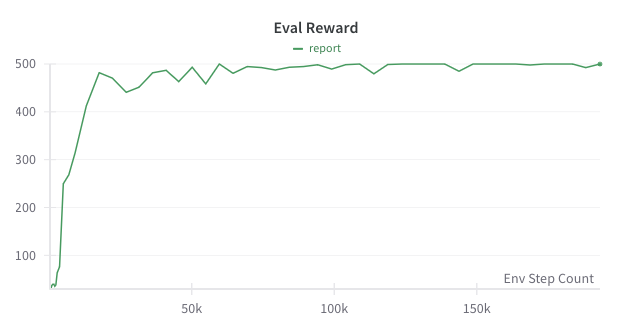
\includegraphics[width=0.8\textwidth]{figures/task1.png}
    \caption{Training curves for the \cartpole environment.}
    \label{fig:cartpole-training-curve}
\end{figure}


\subsection{Analyze each Technique}
